\documentclass[a4paper,10pt,reqno]{amsart}

\makeatletter
\def\specialsection{\@startsection{section}{1}%
  \z@{\linespacing\@plus\linespacing}{.5\linespacing}%
  {\bfseries\centering}}
\def\section{\@startsection{section}{1}%
  \z@{.7\linespacing\@plus\linespacing}{.5\linespacing}%
  {\bfseries\scshape\centering}}
\makeatother

\newenvironment{nouppercase}{%
  \let\uppercase\relax%
  \renewcommand{\uppercasenonmath}[1]{}}{}


\usepackage[utf8]{inputenc}
\usepackage[foot]{amsaddr}
\usepackage{amsmath,amsfonts,amssymb,amsthm,mathrsfs,bm}
\usepackage[margin=0.7in]{geometry}
\usepackage{color}
\usepackage[dvipsnames]{xcolor}
\usepackage{multicol}
\usepackage{soul}

\usepackage{etoolbox}

% Modifications to amsart ToC-related macros...
\makeatletter
\let\old@tocline\@tocline
\let\section@tocline\@tocline
% Insert a dotted ToC-line for \subsection and \subsubsection only
\newcommand{\subsection@dotsep}{4.5}
\newcommand{\subsubsection@dotsep}{4.5}
\patchcmd{\@tocline}
  {\hfil}
  {\nobreak
     \leaders\hbox{$\m@th
        \mkern \subsection@dotsep mu\hbox{.}\mkern \subsection@dotsep mu$}\hfill
     \nobreak}{}{}
\let\subsection@tocline\@tocline
\let\@tocline\old@tocline

\patchcmd{\@tocline}
  {\hfil}
  {\nobreak
     \leaders\hbox{$\m@th
        \mkern \subsubsection@dotsep mu\hbox{.}\mkern \subsubsection@dotsep mu$}\hfill
     \nobreak}{}{}
\let\subsubsection@tocline\@tocline
\let\@tocline\old@tocline

\let\old@l@subsection\l@subsection
\let\old@l@subsubsection\l@subsubsection

\def\@tocwriteb#1#2#3{%
  \begingroup
    \@xp\def\csname #2@tocline\endcsname##1##2##3##4##5##6{%
      \ifnum##1>\c@tocdepth
      \else \sbox\z@{##5\let\indentlabel\@tochangmeasure##6}\fi}%
    \csname l@#2\endcsname{#1{\csname#2name\endcsname}{\@secnumber}{}}%
  \endgroup
  \addcontentsline{toc}{#2}%
    {\protect#1{\csname#2name\endcsname}{\@secnumber}{#3}}}%

% Handle section-specific indentation and number width of ToC-related entries
\newlength{\@tocsectionindent}
\newlength{\@tocsubsectionindent}
\newlength{\@tocsubsubsectionindent}
\newlength{\@tocsectionnumwidth}
\newlength{\@tocsubsectionnumwidth}
\newlength{\@tocsubsubsectionnumwidth}
\newcommand{\settocsectionnumwidth}[1]{\setlength{\@tocsectionnumwidth}{#1}}
\newcommand{\settocsubsectionnumwidth}[1]{\setlength{\@tocsubsectionnumwidth}{#1}}
\newcommand{\settocsubsubsectionnumwidth}[1]{\setlength{\@tocsubsubsectionnumwidth}{#1}}
\newcommand{\settocsectionindent}[1]{\setlength{\@tocsectionindent}{#1}}
\newcommand{\settocsubsectionindent}[1]{\setlength{\@tocsubsectionindent}{#1}}
\newcommand{\settocsubsubsectionindent}[1]{\setlength{\@tocsubsubsectionindent}{#1}}

% Handle section-specific formatting and vertical skip of ToC-related entries
% \@tocline{<level>}{<vspace>}{<indent>}{<numberwidth>}{<extra>}{<text>}{<pagenum>}
\renewcommand{\l@section}{\section@tocline{1}{\@tocsectionvskip}{\@tocsectionindent}{}{\@tocsectionformat}}%
\renewcommand{\l@subsection}{\subsection@tocline{1}{\@tocsubsectionvskip}{\@tocsubsectionindent}{}{\@tocsubsectionformat}}%
\renewcommand{\l@subsubsection}{\subsubsection@tocline{1}{\@tocsubsubsectionvskip}{\@tocsubsubsectionindent}{}{\@tocsubsubsectionformat}}%
\newcommand{\@tocsectionformat}{}
\newcommand{\@tocsubsectionformat}{}
\newcommand{\@tocsubsubsectionformat}{}
\expandafter\def\csname toc@1format\endcsname{\@tocsectionformat}
\expandafter\def\csname toc@2format\endcsname{\@tocsubsectionformat}
\expandafter\def\csname toc@3format\endcsname{\@tocsubsubsectionformat}
\newcommand{\settocsectionformat}[1]{\renewcommand{\@tocsectionformat}{#1}}
\newcommand{\settocsubsectionformat}[1]{\renewcommand{\@tocsubsectionformat}{#1}}
\newcommand{\settocsubsubsectionformat}[1]{\renewcommand{\@tocsubsubsectionformat}{#1}}
\newlength{\@tocsectionvskip}
\newcommand{\settocsectionvskip}[1]{\setlength{\@tocsectionvskip}{#1}}
\newlength{\@tocsubsectionvskip}
\newcommand{\settocsubsectionvskip}[1]{\setlength{\@tocsubsectionvskip}{#1}}
\newlength{\@tocsubsubsectionvskip}
\newcommand{\settocsubsubsectionvskip}[1]{\setlength{\@tocsubsubsectionvskip}{#1}}

% Adjust section-specific ToC-related macros to have a fixed-width numbering framework
\patchcmd{\tocsection}{\indentlabel}{\makebox[\@tocsectionnumwidth][l]}{}{}
\patchcmd{\tocsubsection}{\indentlabel}{\makebox[\@tocsubsectionnumwidth][l]}{}{}
\patchcmd{\tocsubsubsection}{\indentlabel}{\makebox[\@tocsubsubsectionnumwidth][l]}{}{}

% Allow for section-specific page numbering format of ToC-related entries
\newcommand{\@sectypepnumformat}{}
\renewcommand{\contentsline}[1]{%
  \expandafter\let\expandafter\@sectypepnumformat\csname @toc#1pnumformat\endcsname%
  \csname l@#1\endcsname}
\newcommand{\@tocsectionpnumformat}{}
\newcommand{\@tocsubsectionpnumformat}{}
\newcommand{\@tocsubsubsectionpnumformat}{}
\newcommand{\setsectionpnumformat}[1]{\renewcommand{\@tocsectionpnumformat}{#1}}
\newcommand{\setsubsectionpnumformat}[1]{\renewcommand{\@tocsubsectionpnumformat}{#1}}
\newcommand{\setsubsubsectionpnumformat}[1]{\renewcommand{\@tocsubsubsectionpnumformat}{#1}}
\renewcommand{\@tocpagenum}[1]{%
  \hfill {\mdseries\@sectypepnumformat #1}}

% Small correction to Appendix, since it's still a \section which should be handled differently
\let\oldappendix\appendix
\renewcommand{\appendix}{%
  \leavevmode\oldappendix%
  \addtocontents{toc}{%
    \protect\settowidth{\protect\@tocsectionnumwidth}{\protect\@tocsectionformat\sectionname\space}%
    \protect\addtolength{\protect\@tocsectionnumwidth}{2em}}%
}
\makeatother

% #1 (default is as required)

% #2

% #3
\makeatletter
\settocsectionnumwidth{2em}
\settocsubsectionnumwidth{2.5em}
\settocsubsubsectionnumwidth{3em}
\settocsectionindent{1pc}%
\settocsubsectionindent{\dimexpr\@tocsectionindent+\@tocsectionnumwidth}%
\settocsubsubsectionindent{\dimexpr\@tocsubsectionindent+\@tocsubsectionnumwidth}%
\makeatother

% #4 & #5
\settocsectionvskip{10pt}
\settocsubsectionvskip{0pt}
\settocsubsubsectionvskip{0pt}

% #6 & #7
% See #3

% #8
\renewcommand{\contentsnamefont}{\bfseries\Large}

% #9
\settocsectionformat{\bfseries}
\settocsubsectionformat{\mdseries}
\settocsubsubsectionformat{\mdseries}
\setsectionpnumformat{\bfseries}
\setsubsectionpnumformat{\mdseries}
\setsubsubsectionpnumformat{\mdseries}

% #10
% Insert the following command inside your text where you want the ToC to have a page break
\newcommand{\tocpagebreak}{\leavevmode\addtocontents{toc}{\protect\clearpage}}

% #11
\let\oldtableofcontents\tableofcontents
\renewcommand{\tableofcontents}{%
  \vspace*{-\linespacing}% Default gap to top of CONTENTS is \linespacing.
  \oldtableofcontents}

\usepackage{mathtools,enumerate,mathrsfs,graphicx}
\usepackage{epstopdf}
\usepackage{hyperref}

\usepackage{latexsym}


\definecolor{CommentGreen}{rgb}{0.0,0.4,0.0}
\definecolor{Background}{rgb}{0.9,0.9,09}
\definecolor{lrow}{rgb}{0.914,0.918,0.922}
\definecolor{drow}{rgb}{0.725,0.745,0.769}
\definecolor{darkGreen}{RGB}{38,178,0}

\usepackage{listings}
\usepackage{textcomp}
\lstloadlanguages{Matlab}%
\lstset{
    language=Matlab,
    upquote=true, frame=single,
    basicstyle=\small\ttfamily,
    backgroundcolor=\color{Background},
    keywordstyle=[1]\color{blue}\bfseries,
    keywordstyle=[2]\color{purple},
    keywordstyle=[3]\color{black}\bfseries,
    identifierstyle=,
    commentstyle=\usefont{T1}{pcr}{m}{sl}\color{CommentGreen}\small,
    stringstyle=\color{purple},
    showstringspaces=false, tabsize=5,
    morekeywords={properties,methods,classdef},
    morekeywords=[2]{handle},
    morecomment=[l][\color{blue}]{...},
    numbers=none, firstnumber=1,
    numberstyle=\tiny\color{blue},
    stepnumber=1, xleftmargin=10pt, xrightmargin=10pt
}

\numberwithin{equation}{section}
\synctex=1

\hypersetup{
    unicode=false, pdftoolbar=true, 
    pdfmenubar=true, pdffitwindow=false, pdfstartview={FitH}, 
    pdftitle={ELE2024 Coursework}, pdfauthor={A. Author},
    pdfsubject={ELE2024 coursework}, pdfcreator={A. Author},
    pdfproducer={ELE2024}, pdfnewwindow=true,
    colorlinks=true, linkcolor=red,
    citecolor=blue, filecolor=magenta, urlcolor=cyan
}


% CUSTOM COMMANDS
\renewcommand{\Re}{\mathbf{re}}
\renewcommand{\Im}{\mathbf{im}}
\newcommand{\R}{\mathbb{R}}
\newcommand{\N}{\mathbb{N}}
\newcommand{\C}{\mathbb{C}}
\newcommand{\lap}{\mathscr{L}}
\newcommand{\dd}{\mathrm{d}}
\newcommand{\smallmat}[1]{\left[ \begin{smallmatrix}#1 \end{smallmatrix} \right]}

%opening
\title[ELE2024 Coursework]{\Huge ELE2024 Control Coursework}

\author[T. Hagan]{\Large Created by Toby Hagan}
\author[L. Quail]{\Large Lorcán Quail}
\author[S. Ullah]{\Large Syed Sana Ullah}

\address[T. Hagan, L. Quail and S. Ullah]{. Email addresses: \href{mailto:thagan03@qub.ac.uk}%
{thagan03@qub.ac.uk},
\href{mailto:lquail270@qub.ac.uk}{lquail270@qub.ac.uk} and \href{mailto:sullah@qub.ac.uk}%
{sullah@qub.ac.uk}}
\thanks{
        Version 0.0.1. Last updated:~\today.}
\begin{document}

\begin{nouppercase}
\maketitle
\end{nouppercase}

\section*{Introduction}

\par Throughout this project, the nature of a system of a wooden ball on an inclined plane connected to a spring and attracted to an electromagnet was investigated. This system is outlined in figure~\ref{fig:A1Diagram}. For part B of this project, Python was used to simulate the experiments performed on the system and the code used is within this \href{https://github.com/Lorcan-Q/Control_Coursework}{github repositry}.

\begin{figure}[h]
\label{fig:A1Diagram}
 \centering
 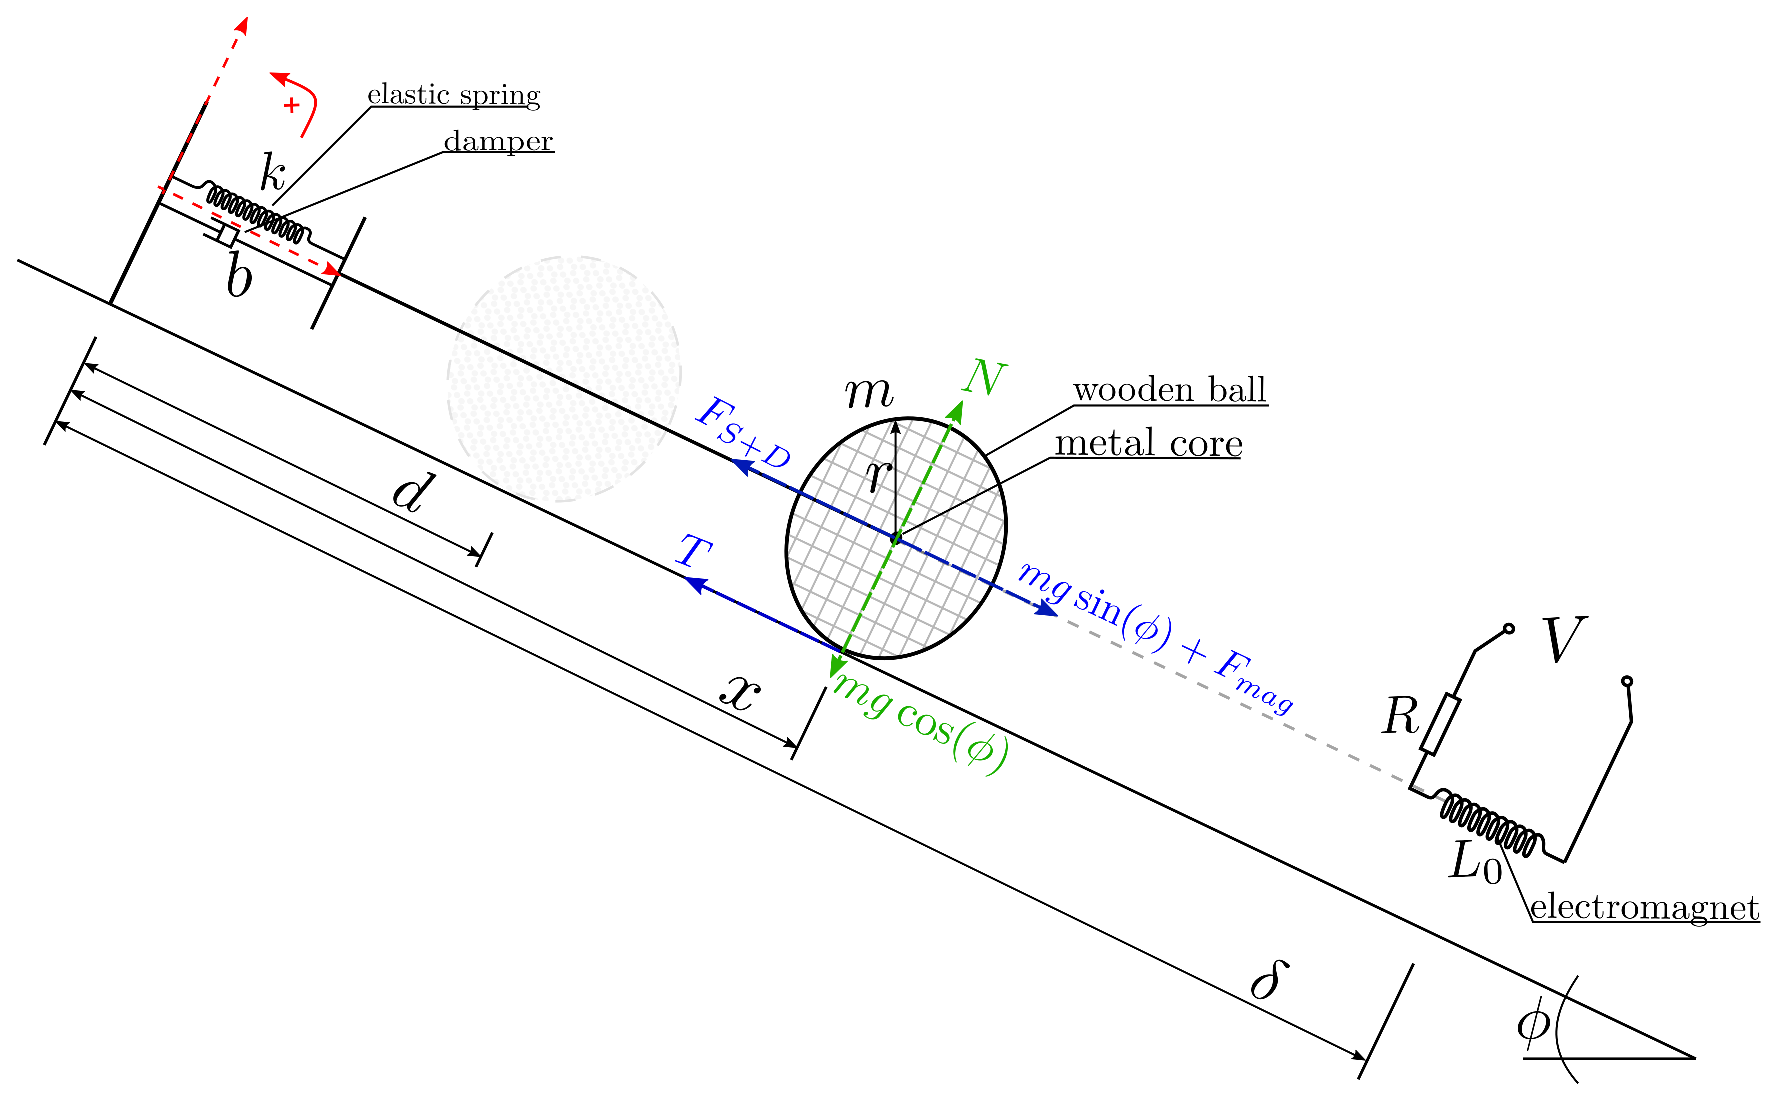
\includegraphics[width=0.6\linewidth]{Figures/FreeBody.eps}
 \caption{System of the wooden ball on an inclined plane with first principles applied.}
\end{figure}

\section{Part A}

\subsection{A1 - System Modelling}\label{sec:A1}

\par To enable the system to be modeled as a set of ordinary differential equations, first principles are applied to the system. Obtaining equations requires the forces acting on the wooden ball be resolved; therefore the vertical forces, i.e. forces acting perpendicular to the slope, can be modelled as:

\begin{equation}
    \color{darkGreen}{N-mg\cos{\phi}=0}\color{black}
\end{equation}


\par Next, the forces working parallel to the slope can be modelled as:

\begin{equation}
\label{eqn:ForcesOrg}
    \color{blue}{mg\sin{\phi}+F_{mag}-T-F_{S+D}=m\ddot{x}}\color{black}
\end{equation}
\\
\par Utilizing figure~\ref{fig:A1Diagram}, $y$ can be defined as $\delta-x$ therefore, the equation for $F_{mag}$ can be written as:
\begin{equation}
    F_{mag} = c(\frac{I}{\delta-x})^2
\end{equation}
\\
\par The torque can be resolved as below in equation~\ref{eqn:torque}.

\begin{align}
    Torque(M)=&-TR=I\ddot{\theta}
    \notag\\
    T =& \frac{-I\ddot{\theta}}{R}
    \label{eqn:torque}
\end{align}

The equation defining the length or a given arc of a circle is defined as $x=R(\theta)$. However, as counter-clockwise rotations are taken as negative in the model and the ball rotates clockwise, the equation results in  $x=R(-\theta)$. Differentiating this equation, $\ddot{\theta}=\frac{\ddot{-x}}{R}$. Thus, the torque can be defined as:

\begin{align}
    T=-\frac{I}{R}(\frac{-\ddot{x}}{R}) = \frac{I\ddot{x}}{R}
    \notag\\
    T = \frac{2mR^2\ddot{x}}{5R^2} = \frac{2m\ddot{x}}{5}
\end{align}
\\
\par The force from the spring and damper can be resolved as:

\begin{equation}
    F_{S+D}=k(x-d)+b\dot{x}
\end{equation}

\par Where $F_{S}=k(x-\delta)$ and $F_D=b\dot{x}$. Finally, the values retrieved for the forces can be plugged into equation~\ref{eqn:ForcesOrg}:

\begin{equation}
    mg\sin{\phi}+c[\frac{I}{\delta-x}]^2-k(x-d)-b\dot{x}=\frac{7m\ddot{x}}{5}
\end{equation}
\\
\par To describe how the input voltage $V$ affects the position $x$ of the ball on the inclined plane, an equation for how the electromagnet behaves can be derived. This is achieved using, $V_{in}=V_R+V_L$, $V_R=RI$ and $V_L=L\dot{I}$

\begin{align}
    V_L&{}={}V_{in}-V_R
    \notag\\
    L\dot{I}&{}={}V-RI
    \notag\\
    \dot{I}&{}={}\frac{1}{L}(V-RI)
    \notag\\
    \dot{I}&{}={}\frac{1}{L_O+L_1e^{-\alpha(\delta-x)}}(V-RI)
\end{align}

The dynamics of the system can be described by the following ordinary differential equations:
\begin{align}
    \frac{7m\ddot{x}}{5}&{}={}mg\sin{\phi}+c[\frac{I}{\delta-x}]^2-k(x-d)-b\dot{x}
    \notag
    \\
    \dot{I}&{}={}\frac{1}{L_O+L_1e^{-\alpha(\delta-x)}}(V-RI)
    \label{eqn:Non-Linear Sys}
\end{align}
\subsection{A2 - State Space Representation}\label{sec:A2}

\parModelling the system in the state space representation will describe the system in terms of its states and inputs. As the model involves terms that are non-linear, utilising the state space representation will enable the linearisation of these terms to be preformed. State variables are created to reduce the ordinary differential equations to the first-order:

\begin{equation}
\label{eqn:state vars}
\bm{z}=
\begin{bmatrix}
z_1
\\
z_2
\\
z_3
\end{bmatrix}
=
\begin{bmatrix}
x
\\
\dot{x}
\\
I
\end{bmatrix}
\end{equation}
\\
Inserting the state variables \ref{eqn:state vars}, into the system equations \ref{eqn:Non-Linear Sys} 
\begin{equation}
    \dot{z_2}=\frac{5}{7m}(mg\sin{\phi}+c[\frac{z_3}{(\delta-z_1)}]-k(z_1-d)-bz_2)
\end{equation}
\begin{equation}
    \dot{z_3}=\frac{V-z_3R}{L_o+L_1^{-\alpha(\delta-x)}}
\end{equation}
\\
The state space representation is defined below, with states $z1, z2, z3$ (defined in \ref{eqn:state vars}) and input V;

\begin{equation}
\bm{\dot{z}}=
\begin{bmatrix}
\dot{z_1}
\\
\dot{z_2}
\\
\dot{z_3}
\end{bmatrix}
=
\begin{bmatrix}
z_2
\\
\frac{5}{7m}(mg\sin{\phi}+c[\frac{z_3}{(\delta-z_1}]-k(z_1-d)-bz_2)
\\
\frac{V-z_3R}{L_o+L_1^{-\alpha(\delta-x)}}
\end{bmatrix}
\end{equation}
\\
\subsection{A3 - Characterising the Equilibrium Point.}\label{sec:A3} 

\par Characterising the equilibrium point: $f(z^e,v^e)=0$

\begin{gather}
    0=z_2^e
    \notag\\
    0=\frac{5}{7m}(mg\sin{\phi}+\frac{c(z_3^e)^2}{(\delta-z_1^e)^2}-k(z_1^e-d)-0)
    \notag\\
    0=\frac{V-z_3R}{L_o+L_1^{-\alpha(\delta-x)}}
\end{gather}

\par As $z_2^e=0$, the term can be omitted from other equations. From this set of equations, $V^e$ can be evaluated as $I^eR$.

\subsection{A4}\label{sec:A4}

\par Subtracting:

\begin{gather}
    \dot{z_1}=z_2-z_2^e
    \\
    \dot{z_2} = \frac{5}{7m}(mg\sin{\phi}+\frac{cz_3^2}{(\delta-z_1)^2}-k(z_1-d)-bz_2)-\frac{5}{7m}(mg\sin{\phi}+\frac{c(z_3^e)^2}{(\delta-z_1^e)^2}-k(z_1^e-d))
    \label{eqn:z_2}\\
    \dot{z_3}=\frac{V-z_3R}{L_o+L_1^{-\alpha(\delta-z_1)}}-\frac{V^e-z_3^eR}{L_o+L_1^{-\alpha(\delta-z_1^e)}}
\end{gather}
\\
\par Next, the only equation that can be simplified is equation~\ref{eqn:z_2} and will be simplified as shown below:

\begin{gather}
    \dot{z_2} = \frac{5}{7m}[c(\frac{z_3^2}{(\delta-z_1)^2}-\frac{(z_3^e)^2}{(\delta-z_1^e)^2})-k(z_1-z_1^e)-bz_2]
\end{gather}

\par Within section A4, the system derived in section~\ref{sec:A3} is linearised at an equilibrium point using derivation variables. The actual values are close to the values at equilibrium during linearisation. This is accomplished by utilising Taylor's approximation theorem, i.e.

\begin{gather}
    \phi(t)=\phi'(t)+(\phi''(t)(x-t)-\phi'(t))+(\frac{\phi^{(3)}(t)}{2!}(x-t)^2-\frac{\phi^{(2)}(t)}{1!}(x-t))+...
    \notag\\
    ...+(\frac{\phi^{(k+1)}(t)}{k!}(x-t)^k - \frac{\phi^{(k)}(t)}{k-1!}(x-t)^k-1) = \frac{\phi^{(k+1)}(t)}{k!}(x-t)^k
\end{gather}
\\
\par Linearise the $\dot{z_2}$ equation then plug the linear equation back into the non-linear equation using Taylor's approximation theorem:


\begin{align}
    \dot{z_2}&=\frac{5c}{7m}(\frac{2z_3^e}{(\delta-z_1^e)^2}(\bar{z_3})+\frac{2(z_3^e)^2}{(\delta-z_1^e)^3}(\bar{z_1}))-\frac{5k}{7m}(\bar{z_1})-\frac{5b}{7m}(\bar{z_2})
    \\
    &=\frac{10cz_3^e}{7m(\delta-z_1^e)^2}(\bar{z_3})+\frac{10c(z_3^e)^2}{7m(\delta-z_1^e)^3}(\bar{z_1})-\frac{5k}{7m}(\bar{z_1})-\frac{5b}{7m}(\bar{z_2})
    \\
    &=\frac{10cz_3^e}{7m(\delta-z_1^e)^2}(\bar{z_3})+\frac{5}{7m}(\frac{2c(z_3^e)^2}{(\delta-z_1^e)^3}-k)(\bar{z_1})-\frac{5b}{7m}(\bar{z_2})
    \\
    &=\color{red}a_1\color{black}\bar{z_3} + \color{red}a_2\color{black}\bar{z_1} - \color{red}a_3\color{black}\bar{z_2}
\end{align}
\\
\par This provides values for \color{red}$a_1$\color{black}, \color{red}$a_2$ \color{black}and \color{red}$a_3$\color{black}

\begin{gather}
    \Psi(z_3,z_1)=\frac{z_3^2}{(\delta-z_1)^2}\approx\Psi_1(z_3^e,z_1^e)+\frac{\delta\Psi}{\delta z_3}\mid_{z_3^e,z_1^e}(z_3-z_3^e)+\frac{\delta\Psi}{\delta z_1}\mid_{z_3^e,z_1^e}(z_1-z_1^e)
    \notag\\
    \frac{\delta\Psi_1}{\delta z_3}=\frac{10cz_3}{7m(\delta-z_1)^2}\color{red}=a_1\color{black}
    \notag\\
    \frac{\delta\Psi_1}{\delta z_1}=\frac{5}{7m}(\frac{2c(z_3)^2}{(\delta-z_1)^3}-k)\color{red}=a_2\color{black}
\end{gather}

\par Next, a value for $\frac{\delta\Psi_2}{\delta z_3}$ must be calculated:

\begin{equation}
    \dot{z_3}=\frac{V-z_3R}{L_o+L_1^{-\alpha(\delta-z_1)}}-\frac{V^e-z_3^eR}{L_o+L_1^{-\alpha(\delta-z_1^e)}}
\end{equation}

\par Insert linearisation for A4 partial derivatives:

\begin{align}
    \dot{z_3}&=\frac{\bar{V}}{L_o+L_1^{-\alpha(\delta-z_1)}}-\frac{R\bar{z_3}}{L_o+L_1^{-\alpha(\delta-z_1^e)}}
    \notag\\
    &=\frac{1}{L_o+L_1e^{\alpha(z_1^e-\delta)}}(\bar{V}-R\bar{z_3})
    \notag\\
    &=\color{red}a_4\color{black}(\bar{V}-R\bar{z_3})
\end{align}

\par Values are then evaluated at zero:

\begin{align} %attempted to save some space by putting the equations next to each other, if it's too messy let me know
    \frac{\delta\Psi}{\delta z_3}\mid_{z_3^e,z_1^e}=\frac{10cz_3^e}{7m(\delta-z_1^e)^2}=a_1,
    &&
    \frac{\delta\Psi}{\delta z_1}\mid_{z_3^e,z_1^e}=\frac{5}{7m}(\frac{2c(z_3^e)^2}{(\delta-z_1^e)^3}-k)=a_2
    \notag\\
    \frac{\delta\Psi_2}{\delta V}\mid_{z_3^e,z_1^e}=\frac{5b}{7m}=a_3,
    &&
    \frac{\delta\Psi_2}{\delta z_3}\mid_{z_3^e,z_1^e}=\frac{1}{L_o+L_1e^{\alpha(z_1^e-\delta)}}=a_4
    \label{eqn:a_4}
\end{align}
\\
%\par However, because $V_e=z_3^eR$, equation~\ref{eqn:a_4} will simply be written as $a_4=0$.

\subsection{A5}\label{sec:A5} 

\par Initially the Laplace transfer function is applied to the linearised system:

\begin{align}
    &\color{darkGreen}(1)\color{black}\;\;\; s\bar{z_1}(s) {}={} s\bar{z_2}(s)
    \\
    &\color{darkGreen}(2)\color{black}\;\;\; s\bar{z_2}(s) {}={} a_1\bar{z_3}+a_2\bar{z_1}-a_3\bar{z_2}
    \\
    &\color{darkGreen}(3)\color{black}\;\;\; s\bar{z_3}(s) {}={} a_4\bar{V}-a_4R\bar{z_3}
    \\
    &\color{darkGreen}(1)\rightarrow(2)\color{black}\;\;\; s(s\bar{z_1}) {}={} a_1\bar{z_3}+a_2\bar{z_1}-a_3\bar{z_2}
    \notag\\
    &\color{darkGreen}(4)\color{black}\;\;\; \bar{z_3} {}={} \frac{z_1(s^2+a_3s-a_2)}{a_1}
    \notag
\end{align}
\\
\par Inserting \color{darkGreen}(4)\color{black}:

\begin{equation}
    \frac{\bar{z_1}}{\bar{V}}=\frac{a_1a_4}{(s+a_4R)(s^2+a_3s-a_2)}\color{red}= G_x\color{black}
\end{equation}
\\

\par This is a third-order transfer function, thus has three poles. This can be modelled using the product of a first and second order transfer function for analytical purposes. Furthermore, the system's response can be approximated using the sum of the responses from the decomposed functions.

\begin{equation}
    G_x = a_1a_4\cdot(\frac{1}{s+a_4R})(\frac{1}{s^2+a^3s-a_2})
\end{equation}

\par Due to the nature of the summation, oscillations present in an impulse reaction from the second-order system would become apparent in the overall system's impulse response. These oscillations would be created due to the second order system being under-damped.
\\
\par A second order transfer function has the form:

\begin{equation}
    G(s) = \frac{k}{\tau^2s^2+2\zeta\tau s+1}
\end{equation}

\par where $k$, $\tau$, $\zeta >$ 0 and $k$ is the static gain, $\zeta$ is the damping factor and $\tau$ is the time constant of the system.
\par An under-damped second order system is categorised by a pair of complex, conjugate, non-real poles. The nature of the poles can be identified by analysing the discriminant of the denominator.

\begin{align*}
    \Delta\tau^2s^2+2\zeta\tau s+1&=(2\zeta\tau)^2 - 4(\tau^2)(1)
    \\
    &=4\zeta^2\tau^2-4\tau^2
    \\
    &=4\tau^2(\zeta^2-1)
\end{align*}

Hence, a damping factor $0 < \zeta < 1$, would create a negative discriminant indicating the system is under-damped due to the presence of a pair of non-real conjugate poles.
\\
\par Equating the second-order transfer function's co-coefficients produces:

\begin{align*}
    \tau^2=1 && 2\zeta\tau&=a_3
    \\
    \tau=1 && 2\zeta&=a_3
    \\
    && \zeta &= \frac{5b}{7m} \cdot \frac{1}{2}
    \\
    && &=\frac{5b}{14m}
\end{align*}

\par The system would present oscillations from an impulse response given that:

\begin{equation}
    0 < \frac{5b}{14m} < 1
\end{equation}
\\

\section{Part B}

%overleaf has an issue with equilibrate however it seems fine to me
\par Due to the forces acting on the system, the ball is only able to equilibrate within a defined space along the plane; utilising the characterised equilibrium points defined in section~\ref{sec:A3}, this space can be defined:

\begin{gather*}
    0=\frac{V^e-z_3^eR}{L_o+L_1^{-\alpha(\delta-z_1^e)}} \rightarrow V^e = z_3^eR
    \\
    0 = \frac{5}{7m}[mg\sin{\phi}+\frac{c(z_3^e)^2}{(\delta-z_1^e)^2}-k(z_1^e-d)]
    \\
    0 = mg\sin{\phi}(\delta-z_1^e)^2 + c(z_3^e)^2 - k(z_1^e-d)(\delta-z_1^e)^2
    \\
    z_3^e = \frac{(\delta-z_1^e)(k(z_1^e-d)-mg\sin{\phi})^\frac{1}{2}}{\sqrt{c}}
\end{gather*}

\par Therefore:

\begin{equation}
\label{eqn:V^e}
    V^e = \frac{R(\delta-z_1^e)(k(z_1^e-d)-mg\sin{\phi})^\frac{1}{2}}{\sqrt{c}}
\end{equation}
\\
\par Evidently from these equations, inputting a value of $z_1^e(x^e) \leq (\frac{mg\sin{\phi}}{k}+d)$ would result in the voltage and current becoming undefined, i.e. resulting in a zero or imaginary value. Furthermore, a value of $z_1^e(x^e) \geq d$ would create a zero or negative result for the equilibrium values which indicate that the electromagnet polarity has switched, thus the ball would not achieve equilibrium. These derivations enable the space to be defined as:

\begin{equation}
    x_{min} < x^e < x_{max}
\end{equation}
\\
\par Where $x_{min} = d + \frac{mg\sin{\phi}}{k}$ and $x_{max} = \delta$
\\
\par Furthermore, using equation~\ref{eqn:V^e}, the ball's equilibrium position at which the equilibrium voltage attains a maximum can be determined.
\\
\begin{figure}[h]
\label{fig:B1Diagram}
 \centering
 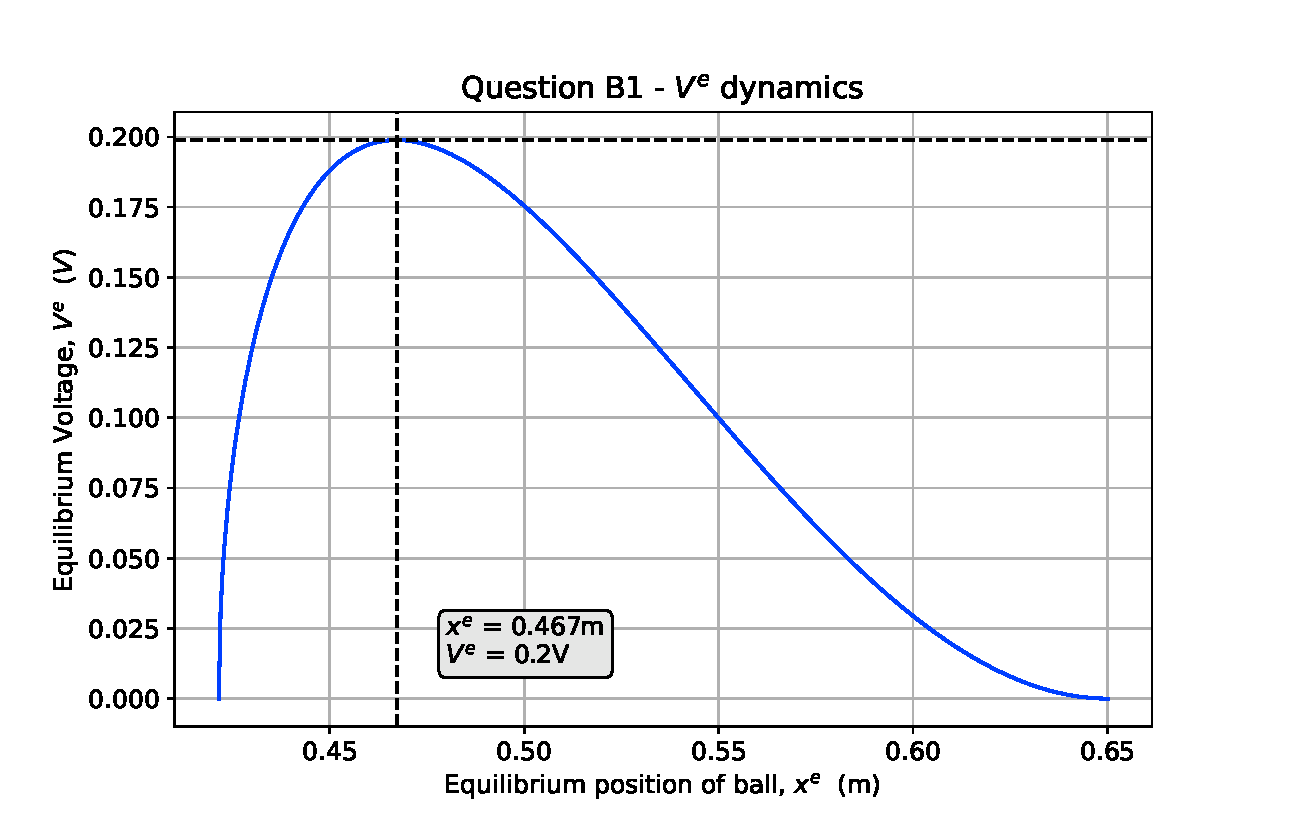
\includegraphics[width=0.6\linewidth]{Figures/B1.eps}
 \caption{Nature of the equilibrium values of $x^e$ and $V^e$ in the system using equation~\ref{eqn:V^e} when simulated in Python.}
\end{figure}

\par As presented in figure~\ref{fig:B1Diagram}, the maximum voltage is approximately equal to 0.2 volts where the equilibrium position is equal to 0.467 metres.

%\begin{lstlisting}[language=python]
%\end{lstlisting}

\end{document}
